
\paragraph{Interpretación económica de la proposición.}
El signo de la derivada \(-a_R/b\) indica cómo aparece una
raíz interior de holgura cuando la innovación cambia de signo.
La raíz \(s=0\) corresponde al extremo con garantía activa,
mientras \(s(h)>0\) permite el régimen de préstamo no restringido
para L. \emph{Exactamente dos raíces de una complementariedad}
no significa exactamente dos equilibrios competitivos: falta
establecer que las 33 variables recuperadas satisfacen, además,
suficiencia individual, todos los mercados y la continuación infinita.
En particular, no se identifica un multiplicador privado con una
variable libre de una estructura Lean sin demostrar la condición
marginal que lo determina.

El lema Lean \texttt{scalar\_complementarity\_exactly\_two} prueba
una equivalencia de soluciones escalares suponiendo monotonicidad
estricta, una raíz positiva y signo positivo en el borde.
No demuestra por sí mismo que el Schur complement del modelo
satisfaga esas condiciones. El resultado del cuerpo conserva
explícitamente la regularidad \(C^1\) y los signos locales como
premisas. El anexo recoge la derivación de las filas, los
Jacobianos y la versión histórica de la comparación S/B.

\section{Resultados numéricos reproducibles}\label{sec:compact_irf}
El experimento fija los mismos estados heredados y la misma
secuencia de innovaciones posteriores para ambas ramas.
Al impacto se perturba \(\epsilon_0^R\) en
\(-10^{-5}\), aproximadamente \(-0.1\) punto básico en la
convención de log tasa, con las demás herramientas constantes.
Las tasas se reportan como \(10^4(R_t-R_t^0)\), sin anualizar,
y las cantidades positivas como \(100\log(x_t/x_t^0)\).
El capital elegido en \(t\) se instala en \(t+1\): no debe
confundirse la producción \emph{corriente} con esa inversión.

\begin{table}[htbp]\centering\small
\caption{Impacto de una innovación inicial de remuneración de reservas de
aproximadamente \(-0.1\) pb. Dos ramas del sistema reducido;
parámetros ilustrativos, no estimaciones.}
\label{tab:compact_impact}
\begin{tabular}{lrr}\toprule
Respuesta al impacto & S & B\\\midrule
Tasa interbancaria (pb) & -0.06363254 & -0.09117145\\
Tasa de crédito (pb) & -0.06363175 & -0.09090760\\
Producción (log \%) & -0.00003580 & -0.00414255\\
Crédito H (log \%) & 0.00109518 & 0.00084065\\
Crédito L (log \%) & -0.00047390 & 0.00157811\\
Pérdida condicional ($100\Delta\log$) & -0.00000248 & 0.00000852\\
\bottomrule\end{tabular}

\end{table}

La caída del costo de crédito y el incremento de préstamos a H
ocurren en ambas ramas. Sin embargo, la pérdida asignativa
\(\mathscr L\) \emph{disminuye} en S y \emph{aumenta} en B.
Esta pérdida compara producción con un referente eficiente
que reasigna factores manteniendo su disponibilidad:
\begin{equation}\label{eq:compact_loss}
\mathscr L_t=
\log\left(\frac{Y^{\mathrm{ef}}_{t+1}}{Y_{t+1}}\right),
\qquad
Y^{\mathrm{ef}}_{t+1}=
\left(\sum_i\nu_i A_i^{1/(1-\alpha-\beta)}\right)^{
1-\alpha-\beta}
 K_{t+1}^{\alpha}L_{t+1}^{\beta}.
\end{equation}
Con masas, tecnología y dotación total de factores comunes
para cada comparación, esta medida es no negativa bajo la
referencia tecnológica indicada. No mide directamente bienestar:
se omiten las ponderaciones de utilidad de trabajadores y
empresarios, costos de inflación y riesgo intertemporal.

\subsection{Por qué más crédito puede coexistir con menos inversión}
La identidad \eqref{eq:compact_capacity} para la firma H
tiene una forma exacta entre referencia y trayectoria perturbada:
\begin{align}
100\Delta\log k_{H,t+1}&=
100\Delta\log(N_{Ht}-c_{Ht})
-100\Delta\log(q_t-H_{Ht}/R_t^L),
\label{eq:compact_decomp_k}\\
100\Delta\log b_{Ht}&=
100\Delta\log H_{Ht}+
100\Delta\log k_{H,t+1}-
100\Delta\log R_t^L.
\label{eq:compact_decomp_b}
\end{align}
El primer componente de \eqref{eq:compact_decomp_k} son recursos
invertibles, no patrimonio bancario. El segundo es la variación
negativa del precio efectivo del capital financiable. Ambas
identidades se calculan \emph{después} de resolver el sistema
conjunto: no son descomposiciones causales con precios fijados.

\begin{table}[htbp]\centering\small
\caption{Componentes exactos del mecanismo empresarial H,
solución reducida no lineal finita de horizonte \(T=640\).
Contribuciones de logaritmos escaladas por 100 y dual normalizado
escalado por \(10^6\).}
\label{tab:compact_mechanism}
% Generated by code/irf/render_mechanism_table.py; do not edit numeric cells by hand.
% T=640 nonlinear finite system, branch-specific reference; values are accounting log contributions.
\begin{tabular}{@{}lrr@{}}\toprule
Magnitud de impacto & Rama S & Rama B\\\midrule
Recursos invertibles $100\Delta\log(N_H-c_H)$ & 0.00002735 & -0.00174198\\
Menor precio efectivo $-100\Delta\log(q-H/R^L)$ & 0.00013674 & 0.00066934\\
\textbf{Capital elegido} $100\Delta\log k_{H,t+1}$ & 0.00016409 & -0.00107264\\
\addlinespace[2pt]
Valor pignorable $100\Delta\log H_H$ & 0.00031268 & 0.00102984\\
Menor tasa $-100\Delta\log R^L$ & 0.00061840 & 0.00088344\\
\textbf{Crédito} $100\Delta\log b_H$ & 0.00109517 & 0.00084064\\
\addlinespace[2pt]
Dual normalizado $10^6\Delta\upsilon_H$ & -1.21674 & 23.08136\\
\bottomrule\end{tabular}

\end{table}

En S los recursos propios netos y el abaratamiento efectivo
contribuyen positivamente al capital. En B domina la contracción
de recursos invertibles, pese al menor costo financiero. Por eso
H puede tomar más crédito pero escoger menos capital; también
el dual normalizado aumenta en B y disminuye en S. Una restricción
activa y un multiplicador de financiación no se intercambian
conceptualmente.

\subsection{Transmisión nominal y producción contemporánea}
La identidad de condiciones de trabajo y consumo, con capital
instalado fijo al impacto, conduce en la parametrización
ilustrativa a
\begin{equation}\label{eq:compact_labor_mechanism}
\Delta\log Y_0
=\frac{\Delta\log m_0-\Delta\log C_0^W}{3}.
\end{equation}
La curva de Phillips con ajuste de precios conecta \(m_0\)
con inflación presente, inflación esperada y actividad futura.
El código reconstruye las contribuciones contemporáneas y
futuras de la identidad, así como la ecuación de Euler del hogar.
El componente futuro puede dominar el contemporáneo incluso
cuando la tasa nominal y real de depósitos disminuyen al inicio.
Estas son identidades evaluadas sobre una solución conjunta,
no choques estructurales adicionales ni experimentos ceteris paribus.

\begin{figure}[p]\centering
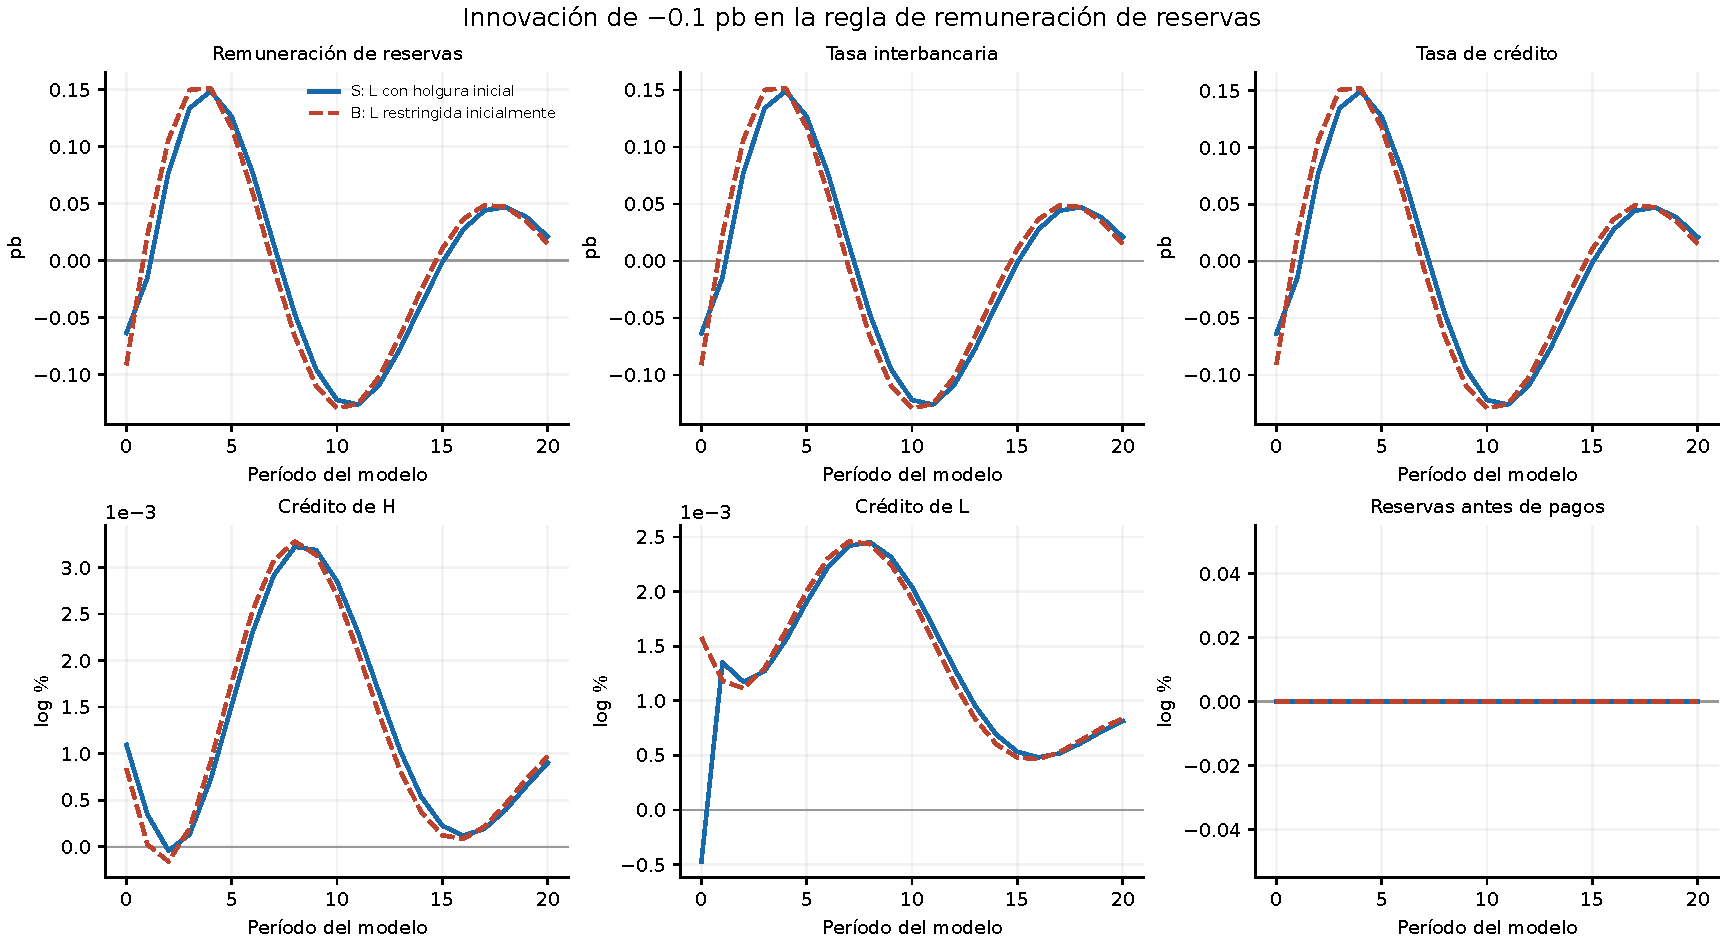
\includegraphics[width=\textwidth]{figures/irf_transmission.pdf}
\caption{Respuestas financieras por rama, reproducidas desde
código y archivos de salida: S y B utilizan las mismas posiciones
heredadas. Las tasas no se anualizan; ninguna trayectoria
constituye una estimación empírica ni un equilibrio infinito
certificado.}
\label{fig:compact_irf_financial}
\end{figure}
\begin{figure}[p]\centering
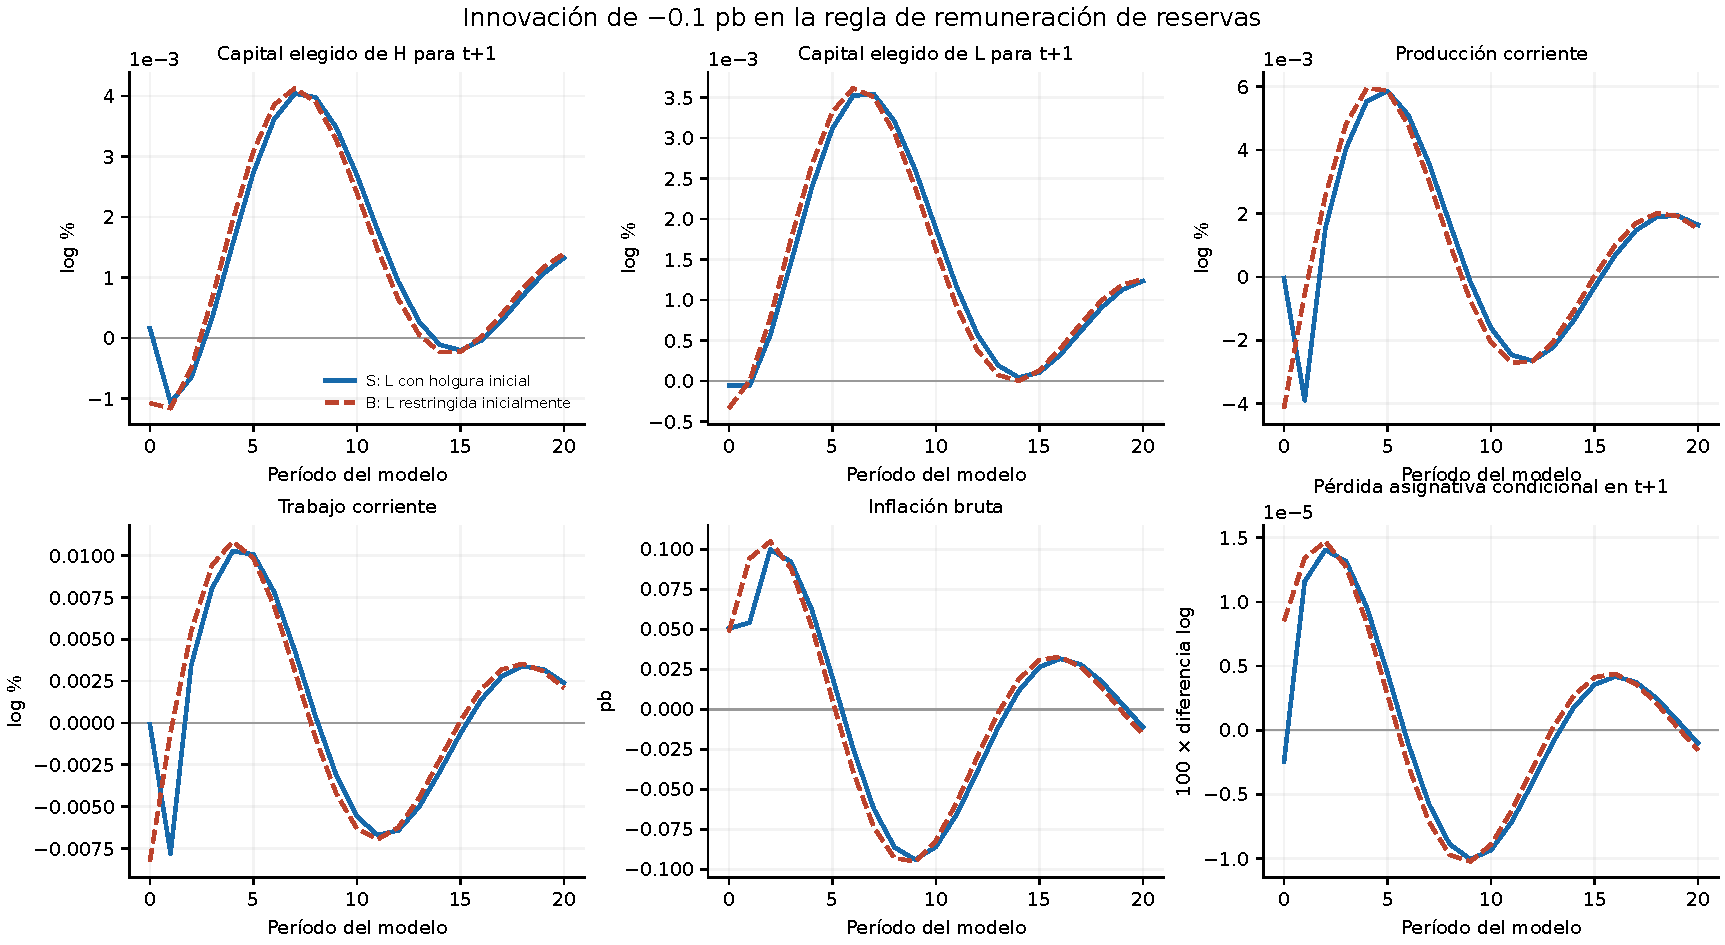
\includegraphics[width=\textwidth]{figures/irf_real_allocation.pdf}
\caption{Capital seleccionado, producción corriente y pérdida
asignativa condicional en las dos ramas. La inversión elegida hoy
se instala mañana, mientras la pérdida usa los recursos del
período siguiente.}
\label{fig:compact_irf_allocation}
\end{figure}

\subsection{Sensibilidad y condiciones de admisibilidad}
El reproductor resuelve el prefijo no lineal y propaga una
gráfica estable \emph{local lineal} desde la fecha dos.
Una auditoría aparte resuelve sistemas no lineales finitos
con horizontes de hasta \(T=640\), bajo cierres terminales
distintos. Las comparaciones reportan residuos, márgenes
de conjunto activo y errores de identidades KKT necesarias.
Cambios en tamaño del shock y paso de Jacobiano preservan
el signo de la producción inicial en los casos ensayados.
Un cierre terminal demasiado cercano puede dar raíces con
signos de régimen inadmisibles; esos ensayos se conservan
como fallos, no se incluyen entre las IRF económicas.

La caída inicial de producción no fue impuesta por el algoritmo,
pero su atribución completa depende de expectativas, consumo
y fijación de precios del sistema. Tampoco está certificado
que la trayectoria con \(h=-10^{-5}\) se encuentre dentro
del radio diminuto de intervención cubierto por los argumentos
intervalares de existencia locales. No usamos la cifra del
radio para defender un experimento de magnitud mayor.

\section{Pruebas, Lean y reproducibilidad}\label{sec:compact_proofs}
La jerarquía de la evidencia es deliberada. Las igualdades
KKT, de presupuesto y de asignación deben examinarse como
fórmulas del modelo fuente; las pruebas aritméticas sobre
coeficientes de un evaluador Python son evidencia numérica
para \emph{ese evaluador}, no automáticamente para Lean.
La auditoría especializada de Lean compiló candidatos que
conectan componentes monetarios (filas 12, 13, 28, 29),
renovación bancaria (6, 22), garantía común (21) y dual
empresarial (33) con sus expresiones fuente bajo premisas
explícitas. También verificó la compatibilidad exacta
\[
a_B=1-\eta_B+\eta_B\psi_B
=\frac{1}{R^L},
\qquad \eta_B=\frac{1}{10},
\quad \psi_B=\frac{10}{R^L}-9,
\]
para la instancia estacionaria correspondiente. La
comparación con Python de siete fórmulas escalares pasó
aritmética intervalar dirigida de 80 cifras. Ninguno de
estos hechos elimina, por sí mismo, la necesidad de
identificar los arreglos externos, las derivadas del operador
económico completo y el calendario de su continuación.

\begin{center}\small
\begin{tabular}{@{}p{2.7cm}p{5.1cm}p{5.0cm}@{}}
\toprule
Objeto & Evidencia disponible & Límite no resuelto\\\midrule
Complementariedad escalar &
Prueba del cuerpo bajo \(C^1\) y signos; lema de orden
formalizado en Lean con premisas visibles &
No certifica que las raíces sean asignaciones
competitivas infinitas.\\
Filas 6, 12, 13, 21, 22, 28, 29, 33 &
Teoremas condicionales sobre expresiones
del operador aumentado, compilados y auditados &
No existe puente de semántica/derivadas de las 34 filas.\\
IRF S/B &
Residuos, sensitividades y KKT necesarias comprobadas
en soluciones finitas &
No se ha demostrado suficiencia dinámica ni
regla de selección de ramas.\\
\bottomrule
\end{tabular}
\end{center}

El comando reproducible de entrada es
\texttt{python code/verify.py}, ejecutado desde la raíz.
El mismo repositorio contiene archivos de entrada,
reproductores de figuras, material Lean, comprobadores
de restricciones, JSON de auditoría y fuentes \LaTeX{}.
Los apéndices conservan las derivaciones históricas
completas y su registro de estatus; no se presenta
un lema más débil como formalización automática
de una proposición más fuerte.

\section{Discusión, límites y agenda de investigación}
\label{sec:compact_discussion}
La \emph{pignorabilidad} \(\theta_i\), la utilización
contractual y el dual de colateral son tres objetos
distintos. Una menor tasa eleva la capacidad para
recursos dados, pero la comparación de equilibrio incluye
precios de capital, consumo, patrimonio bancario y
expectativas. Por ello no sería correcto inferir que
toda expansión de reservas o reducción de remuneración
reduce la mala asignación. Un resultado sobre producción
a dotaciones dadas tampoco prueba mejoras de bienestar.

Nuestra implementación permite conceptualizar remuneración
de reservas, cantidad, coeficiente de encaje, corredor y
operaciones de balance del banco central, pero el
experimento reproducido a lo largo del tiempo
corresponde \emph{solo} a remuneración.
La heterogeneidad de firmas y la garantía robusta son
primitivas modeladas, no estimadas; la economía
recurrente a horizonte infinito y la determinación
del equilibrio requieren una verificación adicional.
La propiedad de crecimiento de largo plazo exigiría
incorporar e identificar el mecanismo de acumulación
persistente y distinguir transiciones de cambios
en la tasa de crecimiento asintótica.

La siguiente prueba estructural necesaria es una
identificación fila por fila del operador de fuente y del
evaluador de intervalos externos, seguida de una demostración
de factibilidad, optimalidad y terminalidad de las
asignaciones recuperadas. Los objetivos generales del programa
de investigación deben tratarse como agenda, no como
resultados que se desprendan de las IRF.

\section{Conclusión}
La interbancaria OTC y la remuneración de reservas
influyen en las condiciones de préstamo, pero la
transmisión hacia inversión depende de las restricciones
y los recursos endógenos de cada empresa. En un sistema
reducido con dos regímenes financieros, la misma innovación
puede aumentar el crédito a la firma más productiva y, aun
así, generar respuestas opuestas de capital y pérdida
asignativa. El resultado analítico central es
\emph{condicional} a las propiedades de una complementariedad
escalar. Las simulaciones ilustran el mecanismo; no
demuestran todavía equilibrio competitivo infinito,
selección de rama, política óptima o crecimiento sostenido.
La distinción es necesaria para interpretar rigurosamente
un modelo monetario con fricciones financieras.
